% The manuscript; compute-limits.pdf beside it is this file built with pdflatex, run three times.
% Every number in it is checked against data/ by code/check_numbers.py.
% Status: draft, shelved on 12 October 2026; not released.
\documentclass[11pt]{article}
\usepackage[letterpaper,margin=1in]{geometry}
\usepackage[T1]{fontenc}
\usepackage{lmodern}
\usepackage{amsmath,amssymb}
\usepackage{array}
\usepackage{booktabs}
\usepackage{graphicx}
\usepackage[font=small,skip=5pt]{caption}
\usepackage{microtype}
\usepackage[hidelinks]{hyperref}

\hypersetup{
  pdftitle={More Compute Is Not Enough: Measured Limits of Self-Training, GPU Throughput and Tracer Scaling on Public Vesuvius Challenge Data},
  pdfauthor={Chase Hendrick}}

\setlength{\emergencystretch}{2em}
\newcommand{\um}{\,\textmu m}

\title{More Compute Is Not Enough: Measured Limits of Self-Training, GPU Throughput and Tracer Scaling on Public Vesuvius Challenge Data}
\author{Chase Hendrick\\[0.2em] {\small Independent Researcher}\\ {\small\href{mailto:chase@hendrickresearch.com}{\texttt{chase@hendrickresearch.com}}}\\ {\small ORCID \href{https://orcid.org/0009-0002-9754-6087}{0009-0002-9754-6087}}}
\date{}

\begin{document}
\maketitle

\begin{abstract}
Reading the carbonized Herculaneum scrolls from X-ray CT is often described as a problem that larger GPUs and longer training will solve. We tested that on our own work for the Vesuvius Challenge, on public data, with rules fixed before each run. For ink detection on PHerc.~841, two rounds of self-training from an ensemble of the released readers led the best released reader, Reader~v2, by $+0.0055$ and $+0.0038$ in pixel AUC on two development segments, against a preregistered gate of $+0.015$. The second round ran on NVIDIA B300 GPUs, cost about $3.3$ times the first, and scored lower. A throughput probe on one B300 showed the training step waiting on data for $43\%$ of its time at batch 16, and that packing up to eight trainings on one card raised no total throughput. An error analysis located the loss: the teacher led Reader~v2 on both segments ($+0.0187$ and $+0.0134$), but the students kept $75\%$ of that lead on one segment and $-23\%$ on the other, and every trained model stayed a near-copy of Reader~v2 (per-pixel Spearman $0.885$ to $0.971$). A plain rank mean of two released readers, with no training, led by $+0.0112$, more than any trained model. For surface tracing, one 60-generation trace with villa's tracer took 960~s on 2 CPU cores, 1494~s on 4 and 2119~s on 8, and ended on the wrong winding every time; holding the seed fixed in the solver, at no extra compute, moved the same trace from a $0.511$ share on the wrong winding to $0.972$ on the right one. Compute did help: it turned a round of nine trainings into an hour and gave a negative answer the day each run was planned. Our reading is that the limits we met are how well training transfers signal, what signal the current readers have at all, and constraints that keep a trace on its sheet, and that compute multiplies good ideas without replacing them.

\medskip
\noindent\textbf{Keywords:} Vesuvius Challenge; Herculaneum papyri; ink detection; self-training; knowledge distillation; GPU throughput; surface tracing; negative results; reproducibility.
\end{abstract}

\section{Introduction}

The Vesuvius Challenge \cite{prizes} asks for software that reads the carbonized Herculaneum scrolls from X-ray CT: trace the papyrus surfaces through the scan, render them flat, and detect the ink, which in the CT of these scrolls is a faint texture rather than a contrast in density \cite{educelab}. Its official pipeline, villa \cite{villa}, ships a surface prediction network, a tracer that grows surfaces from seeds, and ink detection models such as \texttt{ink\_9um} \cite{ink9um}, from which community fine-tunes such as Reader~v2 \cite{readerv2} and d9v2 \cite{d9v2} were built. GPUs that would have been out of reach for an independent researcher a few years ago can now be rented by the minute, and it is tempting to think the remaining problems give way to more of them: train longer, train more models, average them, grow surfaces on more cores. Sutton's ``bitter lesson'' \cite{sutton} is often cited for this view, that general methods that scale with computation win in the long run.

This paper reports what more compute did and did not do on two problems we worked on during 11 and 12 October 2026, with every run on public data and every bar fixed before the run. Section~\ref{sec:setting} sets out the data, the metric and the rules. Section~\ref{sec:ink} reports two rounds of self-training an ink detection model on unlabelled CT, the second on NVIDIA B300 GPUs. Section~\ref{sec:probe} measures what a B300 did during that training. Section~\ref{sec:loss} locates where the gain was lost. Section~\ref{sec:trace} turns to surface tracing on CPU cores, and Section~\ref{sec:integrity} to a data fault that faster fetching does not avoid. Section~\ref{sec:helped} lists where compute did help. Section~\ref{sec:controls} gives the controls and checks, and Section~\ref{sec:discussion} discusses what is and is not shown.

Every statement is labelled: \emph{measured} (a number from a run, with the file it is in), \emph{sourced} (from a cited page, read on the stated date), or \emph{interpretation}. No ink map in this paper is a reading of text, and nothing here concerns a scroll that is eligible for a prize.

\section{Data, metric and rules}\label{sec:setting}

\paragraph{Data (sourced).} PHerc.~841 has been scanned at 9.366\um\ (scan \texttt{20250821151531}) and has three segments with published ink labels in the Challenge's open data: w00, ag896 and ag405 \cite{opendata}. None of the readers compared here was trained on PHerc.~841. w00 and ag896 are one sheet traced twice (measured from the published meshes and supervision masks); they are the development pair. ag405 is the held-out test, to be read once and only after a development pass; it was not read for anything in this paper.

\paragraph{Metric.} Pixel AUC inside the published supervision mask: the probability that a labelled ink pixel scores above a labelled background pixel. It is computed under two label registrations: as stored, and the \emph{texture registration}, in which the labels are moved by $(-6, -7)$ pixels, an offset measured from the CT texture without any model. The texture registration is primary. Every map is also scored with its surface volume in reversed depth order; that \emph{reverse control} should score near $0.5$, and a forward map must beat it clearly.

\paragraph{Baselines (measured).} Reader~v2 scores $0.8788$ on w00 and $0.8308$ on ag896 (texture registration), a mean of $0.8548$; d9v2 scores $0.8763$ and $0.8293$, a mean of $0.8528$.

\paragraph{Rules, fixed before each run.} An arm's three seed maps are averaged. The arm with the best development mean is chosen. It earns the one read of ag405 only if it leads the better baseline by at least $0.015$ under the texture registration and by more than $0$ as stored. On ag405 it would then have to lead by at least $0.02$ under both registrations to count as a better reader. On development terms, that final bar is $0.8748$. The rules were committed to the repository before any map of the round existed.

\paragraph{Machines.} GPU work ran on Modal \cite{modalpricing}: NVIDIA L4s for round~1 and B300s, with B200, H200 and H100 as fallbacks, for round~2 and the probe. Tracing ran on reserved CPU cores. B300 time cost 7.10~USD per hour (sourced, \cite{modalpricing}, read on 12 October 2026).

\section{Two rounds of self-training}\label{sec:ink}

\paragraph{Before the B300s (measured).} Before these rounds, 54 fine-tuned checkpoints of the released readers had been scored on development without one clearing the bar. A fine-tune on training labels re-registered to their CT failed its fresh test, at $0.8573$ as stored against Reader~v2's $0.8595$.

\paragraph{The recipe.} The teacher is an ensemble of the released readers: Reader~v2 and d9v2, each at three windows of depth through the surface volume. On development it scores $0.8975$ on w00 and $0.8442$ on ag896, a mean of $0.8709$ and a lead of $+0.0161$ over Reader~v2 (measured). Its maps of the unlabelled papyrus of w00 and ag896 became pseudo-labels: 92 tiles of 384 pixels over 9.2~cm$^2$, taken only more than 40 voxels from ag405's mesh and from every labelled pixel. Students start from Reader~v2 and train on human ink labels from other scrolls, mixed with the pseudo-label tiles. Round~1 (L4s) had three arms: S0, a control with no pseudo-label tiles; S1, with pseudo-label tiles in half of all draws; and S2, as S1 with a weaker anchor to the starting weights. Round~2 (B300s, twice the steps, 6000 at batch 16) had V1, as S1 with no anchor on pseudo-label patches; V2, with pseudo-label tiles in $80\%$ of draws; and V3, with pseudo-label tiles only. Each arm had three seeds.

\begin{table}[ht]
\centering\small
\begin{tabular}{@{}lrrrr@{}}
\toprule
Map (texture registration) & w00 & ag896 & Mean & Lead over Reader v2 \\
\midrule
Reader v2 & 0.8788 & 0.8308 & 0.8548 & \\
d9v2 & 0.8763 & 0.8293 & 0.8528 & $-0.0020$ \\
Round 1, S0 (no pseudo-labels) & 0.8861 & 0.8281 & 0.8571 & $+0.0023$ \\
Round 1, \textbf{S1} (chosen) & 0.8929 & 0.8277 & 0.8603 & $\mathbf{+0.0055}$ \\
Round 1, S2 & 0.8919 & 0.8199 & 0.8559 & $+0.0011$ \\
Round 2, \textbf{V1} (chosen) & 0.8926 & 0.8246 & 0.8586 & $\mathbf{+0.0038}$ \\
Round 2, V2 & 0.8927 & 0.8227 & 0.8577 & $+0.0029$ \\
Round 2, V3 & 0.8801 & 0.8175 & 0.8488 & $-0.0060$ \\
Teacher, reader ensemble & 0.8975 & 0.8442 & 0.8709 & $+0.0161$ \\
\bottomrule
\end{tabular}
\caption{Development AUC of the self-trained students (measured; \texttt{data/selftrain\_rounds.json}, teacher from \texttt{data/error\_analysis.json}). Each student row is the mean map of three seeds.}
\label{tab:rounds}
\end{table}

\paragraph{Results (measured).} Table~\ref{tab:rounds} and Figure~\ref{fig:leads}. Round~1 chose S1, $+0.0055$ over Reader~v2 ($+0.0056$ as stored); round~2 chose V1, $+0.0038$ ($+0.0032$ as stored). Both are under the $0.015$ gate, so ag405 stayed unread. Round~2 cost 18.84~USD against round~1's 5.68~USD and scored $0.0017$ lower. Pure distillation (V3) lost on both segments and raised its reverse control to $0.605$, against V1's $0.554$. Every arm of both rounds gained on w00 and lost on ag896 against Reader~v2. After round~2, 72 fine-tuned checkpoints had been scored on development.

\begin{figure}[ht]
\centering
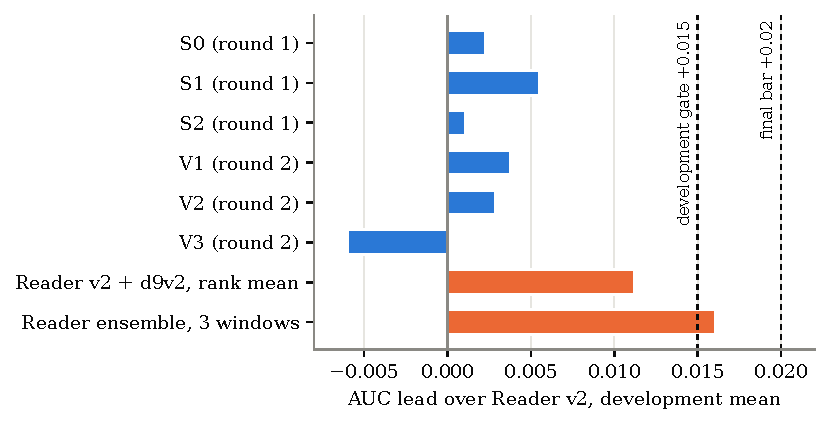
\includegraphics[width=0.9\linewidth]{figures/leads.pdf}
\caption{Development lead over Reader~v2 of each self-trained arm (blue) and of two ensembles of released readers made without training (orange), against the development gate and the final bar (measured; drawn by \texttt{code/make\_figures.py} from \texttt{data/}).}
\label{fig:leads}
\end{figure}

\paragraph{Cost (measured).} The ink line's Modal runs on 12 October cost 29.16~USD in all, by the per-app reports in \texttt{data/costs.json}: the re-registered fine-tune 3.18, round~1 5.94, round~2 18.84, the probe of Section~\ref{sec:probe} 1.10, and a third round stopped in its speed test 0.10. None produced a reader past the gate.

\section{What the GPU was doing}\label{sec:probe}

Round~2's trainings took about 11 minutes each for 6000 steps at batch 16. A throughput probe on one B300 (1.10~USD) timed the training step alone on data already on the GPU, the data loader alone, and the real training script (measured; \texttt{data/b300\_probe.json}; NVIDIA B300 SXM6 AC, PyTorch 2.14.1, CUDA 13.2).

\begin{table}[ht]
\centering\small
\begin{tabular}{@{}lrr@{}}
\toprule
 & Batch 16 & Batch 64 \\
\midrule
GPU step alone (s) & 0.0374 & 0.0934 \\
Real training step (s) & 0.0655 & 0.1214 \\
Share of the real step spent waiting on data & 0.43 & 0.23 \\
GPU busy during real training & $52\%$ & $74\%$ \\
Real patches per second & 244 & 527 \\
\bottomrule
\end{tabular}
\caption{One B300 running the real training step and the same step alone (measured). The waiting share is one minus the ratio of the two step times.}
\label{tab:probe}
\end{table}

\paragraph{Results (measured).} Table~\ref{tab:probe} and Figure~\ref{fig:probe}.
\begin{itemize}
\item Bigger batches buy less than they appear to. Alone, the step goes from 428 patches per second at batch 16 to 812 at batch 256: $1.9$ times the throughput for 16 times the batch.
\item Packing trainings on one card bought nothing. One, two, four and eight copies of the batch-16 step running together delivered 424, 402, 402 and 403 patches per second in total, while the card's reported busy share rose from $40\%$ to $79\%$.
\item More loader workers stopped helping early, then hurt. At batch 16 the threaded loader gave 2.7 batches per second with one thread and 36 with eight, and stayed between 37 and 39 from 16 to 44 threads. Forked processes peaked at 52 batches per second with 16 workers and fell to 26 with 44. At batch 64 the threaded loader gave about 9 batches per second at every count from 8 to 44, close to the real step's 8.2.
\item An online teacher costs twice the step. Running the frozen network six times per step, as a live six-map teacher would, took 0.080~s at batch 16 against 0.037~s.
\end{itemize}

\begin{figure}[ht]
\centering
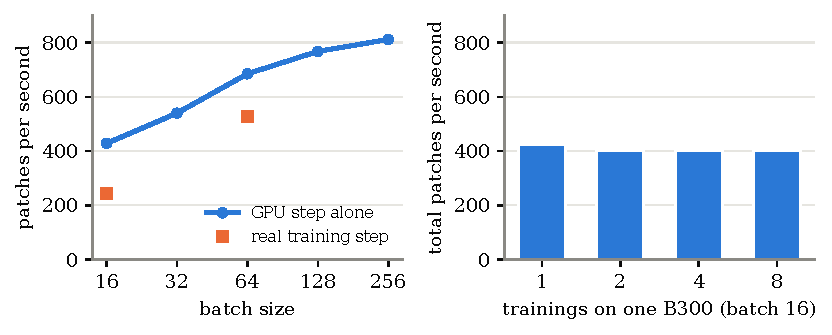
\includegraphics[width=0.9\linewidth]{figures/probe.pdf}
\caption{Left: patches per second on one B300 for the training step alone (blue) and the real training step with its loader (orange). Right: total patches per second with one to eight trainings sharing the card (measured).}
\label{fig:probe}
\end{figure}

\paragraph{Interpretation.} At batch 64 the threaded loader alone sets the pace. At batch 16 the loader alone delivers more batches than the step needs (37 against 27), yet the real step runs at 15; the loss is in how loading and training share the machine, not in the loader's raw speed. A better loader would make the same rounds roughly twice as fast. It would not change what they learned: a perfectly fed B300 trains the same students sooner.

\section{Where the gain was lost}\label{sec:loss}

An error analysis of the development maps, each number re-derived by an independent check with its own code, located the loss (measured; \texttt{data/error\_analysis.json}).

\paragraph{The teacher had the signal on both segments (measured).} The reader ensemble led Reader~v2 by $+0.0187$ on w00 and $+0.0134$ on ag896. Averaging two lineages of readers over three depth windows does fix part of what Reader~v2 gets wrong on ag896.

\paragraph{The students did not carry it over (measured).} S1 kept $75\%$ of the teacher's lead on w00, $-23\%$ on ag896 and $34\%$ on the mean. Its per-pixel rank change against Reader~v2 correlates $0.727$ and $0.708$ with that of S0, the plain fine-tune, and only $0.457$ and $0.369$ with that of the reader average. Bootstrapped over 107-pixel blocks (2000 draws), S1's lead is $+0.0141$ on w00 ($95\%$ interval $0.0051$ to $0.0229$) and $-0.0031$ on ag896 ($-0.0116$ to $0.0059$).

\paragraph{Every trained model is a near-copy of Reader~v2 (measured).} Per-pixel Spearman correlation with Reader~v2 is $0.885$ to $0.971$ for the fine-tunes and $0.983$ to $0.993$ between seeds of S1, against $0.676$ and $0.858$ between Reader~v2 and d9v2 on w00 and ag896. A seed ensemble differs from its best seed by $-0.0003$ to $+0.0008$.

\paragraph{No training beats a plain average (measured).} A rank mean of Reader~v2 and d9v2, with no training, scores $0.8931$ and $0.8389$, a mean of $0.8660$ and a lead of $+0.0112$, more than any trained model. Outside the windows examined in earlier rounds its lead holds ($+0.0126$, interval $0.0044$ to $0.0218$) while S1's shrinks to $+0.0043$. An ensemble built only from the Reader~v2 line adds at most $+0.0014$ over S1.

\paragraph{Nothing that exists reaches the final bar (measured).} Of 13{,}058 ensemble and post-processing settings searched in-sample, none reaches $0.8748$; the best scores $0.8724$, and $0.8674$ without blur. These were tuned on the data they are scored on, so they are optimistic.

\paragraph{A shared floor (measured).} In 25 blocks of 107 pixels (13 on w00, 12 on ag896) where all five checked models score below $0.65$, holding $10.9\%$ and $12.5\%$ of all ink and background pairs, each model loses $20\%$ to $24\%$ of its deficit. The blocks were chosen because all five fail there, so part of that equal cost is by construction.

\paragraph{Not the labels' alignment (measured).} The best common label offset gains $0.0006$ to $0.0010$ over the texture registration, and S1's lead stays between $0.0033$ and $0.0062$ under every registration tried. Leaving out a 5-pixel ring at the label edges lifts every model, Reader~v2 to $0.8752$ and S1 to $0.8799$, and narrows S1's lead from $0.0055$ to $0.0047$.

\paragraph{Interpretation.} The round-2 B300 run made the same students faster, and they kept the same small part of their teacher's gain. The limit was how training transferred the teacher's signal into one network and, beyond that, signal no current reader has: the shared floor. A faithful copy of the current teacher can at best approach $+0.016$; to pass $+0.02$ a model must be right where both released readers are wrong, which calls for a different lineage, different inputs or different training data. This matches what is known about pseudo-labelling, in which a student fits its teacher's mistakes along with its knowledge \cite{arazo}, and about distillation, where what transfers depends on the training signal more than on its length \cite{hinton, noisystudent}.

\section{Surface tracing on more cores}\label{sec:trace}

villa's tracer, \texttt{vc\_grow\_seg\_from\_seed}, grows a surface one generation at a time from a seed point on the surface prediction and re-solves it as it grows.

\paragraph{More cores, slower (measured).} One trace on PHerc.~139 (scan \texttt{20250728140407}, 9.362\um, the published surface prediction and normal grids), from a seed on the published winding w031, 60 generations, was repeated with reserved CPU cores on Modal on 11 October 2026 (\texttt{data/tracer\_cores.json}, Figure~\ref{fig:tracer}). It took 960~s on 2 cores, 1494~s on 4 and 2119~s on 8; a 16-core run did not finish. Each finished run covered the same 4.88~cm$^2$ and ended mostly on the neighbouring winding w033, with a dominant share of $0.511$, $0.516$ and $0.430$.

\begin{figure}[ht]
\centering
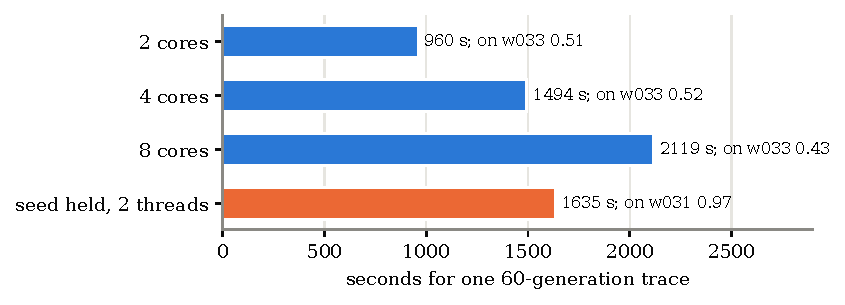
\includegraphics[width=0.9\linewidth]{figures/tracer.pdf}
\caption{Wall time of one 60-generation trace by reserved cores (blue) and with the seed held fixed (orange), with the winding each trace mostly lies on and its share within 4 voxels (measured; the anchored run is from \cite{issue2059, pr2063}, on a different machine).}
\label{fig:tracer}
\end{figure}

\paragraph{A constraint instead of compute (measured).} The trace was on the wrong winding from its first step. The four vertices the tracer places at the seed are free in every solve, so a seed $1.1$ voxels from w031 and $24.5$ from w033 ended its first 10 generations with all four seed vertices, and 265 of 324 vertices, on w033, $25.3$ voxels from the seed, while the run's metadata still recorded the seed \cite{issue2059}. Holding one vertex fixed at the seed in every solve \cite{pr2063}, on the same seed, 60 generations and 2 threads, gave the same 4.88~cm$^2$ with a $0.972$ share on w031 and 4.74~cm$^2$ on it, against $0.511$ on w033 and none on w031 without the anchor (\texttt{data/seed\_anchor.json}). The anchored run took 1635~s against 960~s; whether the anchor or the machine accounts for that is not known.

\paragraph{Interpretation.} The tracer's work is sequential: each generation depends on the one before, so more cores add coordination and little parallel work, as Amdahl's law predicts for a mostly serial job \cite{amdahl}. Independent traces do run side by side, and we used that (Section~\ref{sec:helped}). But the wrong winding was not a shortage of iterations; a correct constraint fixed it and cost more time, not less. What remains after the anchor, in our experience, is telling touching sheets apart: where sheets press together, a trace can cross from one to the next while every vertex stays close to some sheet of the prediction. That is a question of signal, the same shape as the shared floor of Section~\ref{sec:loss}. It is one seed on one scroll, and PHerc.~139 is a development scroll with published windings.

\section{A fault that faster fetching does not avoid}\label{sec:integrity}

\paragraph{Measured.} From one cloud machine on 8 October 2026, the Challenge's open-data bucket answered HTTP~404 for chunks it holds: 102 of 316 requests with 32 workers, 16 of 80 with one worker, 19 of 60 from separate processes, none of 60 on one reused connection and none of 1580 HEAD requests (\texttt{data/false404.json}, \cite{issue2058}). VC3D caches any 404 as an empty chunk and serves it as zeros from then on, so a fresh render of a crop of the PHerc.~139 segment w035 came out with $27.7\%$ zero samples, exit code 0 and no warning; removing the false cache entries brought that to $0.03\%$. The fix \cite{pr2060} counts a 404 as missing only when S3 says the key does not exist, and retries otherwise.

\paragraph{Interpretation.} More workers did not avoid the fault, and a pipeline that fetches faster only writes holes into its renders sooner. On scroll data a hole of zeros looks like blank papyrus, so the error is silent downstream. Throughput is worth nothing until the inputs are right.

\section{Where compute did help}\label{sec:helped}

\begin{itemize}
\item \emph{Wall clock per round (measured).} Round~1 ran nine trainings and their maps in about 50 minutes on L4s. Round~2 ran its trainings in parallel on B300s at about 11 minutes each after a pilot. A round that would take a day on one card took under an hour.
\item \emph{Fast answers to engineering questions (measured).} The probe answered whether the card was starved in one short run for 1.10~USD, before a wider round spent more.
\item \emph{Fast falsification (measured).} Two self-training rounds and a fine-tune on re-registered labels each reached a verdict on the day they were planned. A negative result that arrives in hours stops a line of work before it costs a week.
\item \emph{Independent work in parallel (interpretation).} One trace cannot use more cores, but many independent traces, seeds or maps can run side by side, each on a small machine.
\end{itemize}

\section{Controls and checks}\label{sec:controls}

\begin{itemize}
\item \emph{Pipeline check (measured).} Before round~1 the scoring pipeline reproduced d9v2's earlier scores on the development crops exactly.
\item \emph{Reverse controls (measured).} Across the error analysis, reverse maps score $0.52$ to $0.62$ and every forward map beats its reverse by $0.19$ to $0.37$.
\item \emph{Held-out data.} ag405 was never read by these students. The self-training rounds stopped at the development gate, as their rules required.
\item \emph{Independent recomputation (measured).} Every number taken from the error analysis was recomputed by a separate check with its own code; findings that check refuted are not used here. One was an earlier figure of about $10\%$ of ag896's labelled background flagged as ink by every model, which at an equal false-positive rate is $4.9\%$ against $3.5\%$ on w00.
\item \emph{A leak, disclosed (measured).} Rounds~1 and~2 kept pseudo-label targets away from development pixels but let PHerc.~841 CT near them into pseudo-label tiles as context. If it had any effect, it more likely favoured the students on development than hurt them (interpretation), so it does not weaken the negative result. Later work blanks that CT.
\item \emph{Tracing references.} Windings are assigned by the nearest published PHerc.~139 winding (w023 to w040) within a distance cut-off. A seed on w027 classifies as w027 and the nearest w033 vertex to the seed classifies as w033 \cite{issue2059}.
\item \emph{Numbers in this paper.} \texttt{code/check\_numbers.py} recomputes every derived number in the tables and text from \texttt{data/} and checks that it appears in this file as printed.
\end{itemize}

\section{Discussion}\label{sec:discussion}

\paragraph{What is shown.} On two development segments of one public scroll, adding compute to self-training from the released readers did not move a reader past a fixed gate, and the round with the faster, dearer hardware scored lower. On one B300, the training step was bound by data and by how loading shares the machine, and packing trainings bought nothing. The gain was lost in transferring the teacher's signal to the student, and a floor of errors shared by every model remains. For tracing, more cores made one trace slower, and a constraint, not compute, put it on the right winding.

\paragraph{What is not shown.} The development pair is one sheet traced twice; the ensembles of Section~\ref{sec:loss} were scored on the data they were chosen on; the tracing results come from one seed on one scroll. We did not train a large new architecture from scratch, gather new labelled data at scale, or use different CT inputs, and compute may well matter for those. A third self-training round and a test of a different reader architecture were under way at the time of writing and are not reported here. Our claim is about adding compute to the methods we had.

\paragraph{Relation to the bitter lesson.} These results do not contradict Sutton \cite{sutton}. His argument is about general methods that keep improving as computation grows, given the data to learn from. Here the data were fixed: two labelled segments for development, and pseudo-labels from readers that share their errors. More computation on the same signal reproduced the same signal faster.

\paragraph{What we would try next.} For ink: training that carries a teacher's gain into the student on every segment, checked by label-free agreement between student and teacher on each segment, and a second lineage or new input that is right where both released readers are wrong, tested on the shared floor. For tracing: a per-vertex signal of which winding a surface is on that holds where sheets touch. For both: correctness first, because a fast pipeline on wrong inputs, or on the wrong winding, produces wrong answers faster.

{\raggedright\noindent\textbf{Data availability.} The numbers behind every table and figure are in \texttt{data/}, with the SHA-256 of the run file each was copied from. \texttt{code/check\_numbers.py} checks this manuscript against them and \texttt{code/make\_figures.py} redraws the figures. The CT, segments and labels are the Vesuvius Challenge's open data \cite{opendata}; the readers are those released by their authors \cite{ink9um, readerv2, d9v2}. Ink maps, weights and scroll data are not included.\par}

\medskip
\noindent\textbf{Acknowledgements.} We thank the Vesuvius Challenge for the open data and tools, and Domenico Russo and TAUIL-Abd-Elilah for releasing Reader~v2 and d9v2.

\noindent\textbf{Rights and licenses.} Copyright \textcopyright\ 2026 Chase Hendrick. The manuscript and figures are all rights reserved. The programs and data in \texttt{code/} and \texttt{data/} are licensed under the Apache License, Version 2.0, subject to component notices.

\noindent\textbf{Use of AI.} This work was prepared with AI assistance. The author takes full responsibility for its content.

\begin{thebibliography}{20}

\bibitem{amdahl} G. M. Amdahl, Validity of the single processor approach to achieving large scale computing capabilities, \emph{AFIPS Conference Proceedings} \textbf{30} (1967) 483--485.

\bibitem{arazo} E. Arazo, D. Ortego, P. Albert, N. E. O'Connor and K. McGuinness, Pseudo-labeling and confirmation bias in deep semi-supervised learning, \emph{International Joint Conference on Neural Networks} (2020); arXiv:1908.02983.

\bibitem{d9v2} TAUIL-Abd-Elilah, d9v2, a fine-tune of \texttt{ink\_9um}, release v1.0 of \url{https://github.com/TAUIL-Abd-Elilah/pherc0826-first-letters-search}, file \texttt{d9v2\_ft-012000.pth} (SHA-256 \texttt{50d2ad0e...a18f966}).

\bibitem{educelab} S. Parsons, C. S. Parker, C. Chapman, M. Hayashida and W. B. Seales, EduceLab-Scrolls: verifiable recovery of text from Herculaneum papyri using X-ray CT, preprint, arXiv:2304.02084 (2023).

\bibitem{hinton} G. Hinton, O. Vinyals and J. Dean, Distilling the knowledge in a neural network, preprint, arXiv:1503.02531 (2015).

\bibitem{ink9um} Vesuvius Challenge, \texttt{ink\_9um}, \url{https://huggingface.co/scrollprize/ink_9um}.

\bibitem{issue2058} C. Hendrick, VC3D caches any HTTP 404 as a missing chunk, villa issue \#2058 (12 October 2026), \url{https://github.com/ScrollPrize/villa/issues/2058}.

\bibitem{issue2059} C. Hendrick, \texttt{vc\_grow\_seg\_from\_seed}: the explicit seed is not held, villa issue \#2059 (12 October 2026), \url{https://github.com/ScrollPrize/villa/issues/2059}.

\bibitem{modalpricing} Modal, Pricing, \url{https://modal.com/pricing} (read 12 October 2026).

\bibitem{noisystudent} Q. Xie, M.-T. Luong, E. Hovy and Q. V. Le, Self-training with Noisy Student improves ImageNet classification, \emph{IEEE/CVF Conference on Computer Vision and Pattern Recognition} (2020); arXiv:1911.04252.

\bibitem{opendata} Vesuvius Challenge, open data, PHerc.~841 and PHerc.~139, \url{https://vesuvius-challenge-open-data.s3.us-east-1.amazonaws.com/} (read October 2026).

\bibitem{pr2060} C. Hendrick, Don't cache an unconfirmed S3 404 as a missing chunk, villa pull request \#2060 (12 October 2026), \url{https://github.com/ScrollPrize/villa/pull/2060}.

\bibitem{pr2063} C. Hendrick, opt-in seed anchor for \texttt{vc\_grow\_seg\_from\_seed}, villa pull request \#2063 (12 October 2026), \url{https://github.com/ScrollPrize/villa/pull/2063}.

\bibitem{prizes} Vesuvius Challenge, Prizes, \url{https://scrollprize.org/prizes} (read 12 October 2026).

\bibitem{readerv2} D. Russo, Reader v2, a fine-tune of \texttt{ink\_9um}, \url{https://huggingface.co/domenicor046/reader-v2}, file \texttt{reader-v2-step040000.pth} (SHA-256 \texttt{654ec5ac...ab5d3a6}).

\bibitem{sutton} R. Sutton, The bitter lesson (13 March 2019), \url{http://www.incompleteideas.net/IncIdeas/BitterLesson.html}.

\bibitem{villa} Vesuvius Challenge, villa, \url{https://github.com/ScrollPrize/villa}.

\end{thebibliography}

\end{document}
